% pdflatex abstract.tex && rm *.aux *.bbl *.blg *.log *.out

\documentclass{article}
\usepackage{geometry}
\usepackage{hyperref}
\usepackage{amsmath}
\usepackage{tikz}
\usepackage{amssymb}
\usepackage{enumitem}
\geometry{a4paper, margin=1in, includefoot}

\usetikzlibrary{positioning,chains, fit, shapes.geometric}

\begin{document}

\title{\texttt{RTPlayground}}
\date{\today}

\maketitle

\section{Background and Motivation}

Training, testing, and comparing RL algorithms require controlled experiments and environmental setup. Unfortunately, there is a lack of uniformity and standardization when it comes to RL training and testing on real world tasks. \textbf{\texttt{RTPlayground} (Robot Training Playground) aims to provide a standardized framework for testing RL algorithms on both simulated and real world experiments}.

Our objective is to provide users with:
\begin{enumerate}[nolistsep]
    \item A standardized API for setting up environments and tasks; logging metrics on both simulated and real world experiments; and environment rollouts on both simulations and real world environments.
    \item The ability to easily compare results between different algorithms and between simulations and real world experiments.
\end{enumerate}

\section{Conceptual Design}

The diagram below illustrates the connection between the various components of the framework.

\begin{figure}[h]
    \centering
    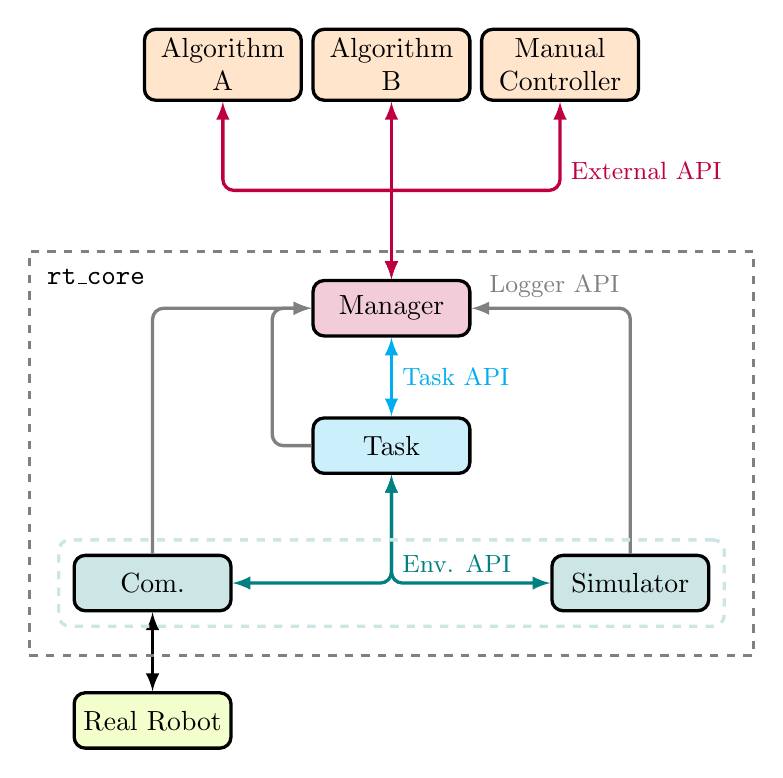
\begin{tikzpicture}[square/.style={rounded corners,regular polygon,regular polygon sides=4, draw,thick}, rect/.style={rounded corners, rectangle, draw,thick, text width = 5em, align=center, minimum height=2em}]

        \node[rect, very thick, fill = purple!20] (manager) {Manager};
        \node[rect, below=of manager, very thick, fill = cyan!20] (task) {Task};
        \node[rect, below left= of task, very thick, fill = teal!20] (driver) {Com.};
        \node[rect, below right = of task, very thick, fill = teal!20] (sim) {Simulator};
        \node[above=of manager] (abvman) {};
        \node[rect, above left= of abvman, very thick, fill = orange!20] (alg1) {Algorithm A};
        \node[rect, above=of abvman, very thick, fill = orange!20] (alg2) {Algorithm B};
        \node[rect, above right = of abvman, very thick, fill = orange!20] (alg3) {Manual Controller};
        \node[rect, below = of driver, very thick, fill = lime!20] (robot) {Real Robot};
        \node[above left= 1.5em of task] (abvtask) {};

        \path[draw, very thick, latex-latex, rounded corners, color = teal] (task) |- (driver);
        \path[draw, very thick, latex-latex, rounded corners, color = teal] (task) |- node[anchor=south west] {\small{Env. API}} (sim);
        \path[draw, very thick, latex-latex, rounded corners, anchor=west, color = cyan] (manager) edge node {\small{Task API}} (task);
        \path[draw, very thick, latex-, rounded corners, color = purple] (manager) -- (abvman.center);
        \path[draw, very thick, latex-, rounded corners, color = purple] (manager) -- (abvman.center);
        \path[draw, very thick, latex-, rounded corners, color = purple] (manager) -- (abvman.center);
        \path[draw, very thick, -latex, rounded corners, color = purple] (abvman.center) -| (alg1);
        \path[draw, very thick, -latex, rounded corners, color = purple] (abvman.center) -| (alg2);
        \path[draw, very thick, -latex, rounded corners, color = purple] (abvman.center) -| node[anchor=south west] {\small{External API}} (alg3);
        \path[draw, very thick, latex-latex, rounded corners] (driver) -- (robot);
        \path[draw, very thick, latex-, rounded corners, color = gray] (manager) -| node[anchor = south east] {\small{Logger API}} (sim);
        \path[draw, very thick, latex-, rounded corners, color = gray] (manager) -| (driver);
        \path[draw, very thick, -, rounded corners, color = gray] (task) -| (abvtask.center);
        \path[draw, very thick, -latex, rounded corners, color = gray] (abvtask.center) |- (manager);
        \node[draw, very thick, rounded corners, fit=(driver) (sim), inner sep = 0.5em, align = left, color = teal!20, dashed] (env) {};

        \node[draw, very thick, dashed, fit=(manager) (env), inner sep = 1.0em, align = left, color = black!50] (core) {};
        \node[below right= 0.5 em of core.north west] {\texttt{rt\_core}};
\end{tikzpicture}
\end{figure}

\subsection{\texttt{rt\_core}: Components and APIs}

\begin{itemize}[nolistsep]
    \item \textbf{Manager Module}: Orchestrates the flow of information from the task and environment modules to the external modules. The manager also provides an interface for a centralized logging system that allow comparison between multiple algorithms
    \item \texttt{RTPlayground} focuses on Markov decision processes (MDP), defined with a 4-tuple $(S, A, T, R)$ where $S$ and $A$ are sets of states and actions, $T$ is the transition probability, and $R$ is the reward function. The following components enables the development of various MDPs for training and testing:
        \begin{itemize}[nolistsep]
            \item \textbf{Task Module}: Configure and output the reward function $r = R(s,a)$, task termination criteria $d = f_{\text{done}}(s,a)$, and initial state probabilities $s_0 \sim S_0$.
            \item \textbf{Environment}: The ``environment" consists of the robot and its environment. The environment is the source of the state transition probability $s' \sim T(s, a)$ and the state-observation mapping $o \sim O(s)$. In order to enable both real world and simulated experiments, the environment module is broken down into two separate modules as follows:
                \begin{itemize}[nolistsep]
                    \item \textbf{Communicator Module}: Communication interface with the real robot.
                    \item \textbf{Simulator Module}: Simulates the robot and provides a standardized communication interface with the simulated robot.
                \end{itemize}
        \end{itemize}
    \item \textbf{External API}: An outward facing API, based on OpenAI Gym's API.
    \item \textbf{Task API}: A standardized API for querying and setting up task modules.
    \item \textbf{Environment API}: A standardized API for interacting and setting up environment modules.
\end{itemize}

\subsection{External Modules}

\begin{itemize}[nolistsep]
    \item \textbf{Training algorithms}
    \item \textbf{Testing algorithms}
    \item \textbf{Data collecting algorithm}: For offline RL, imitation learning, etc.
    \item \textbf{Manual control modules}: For manually controlling robot via a user interface.
\end{itemize}

\end{document}
